\chapter{Fonction carrée}
\section{Fonction carrée}

\begin{definition}[Fonction carrée]
  La fonction définie sur $\mathbb R$ par $f(x)=x^2$ est appelée \emph{fonction carrée}.
\end{definition}

\begin{propriete}[Variations]
  Le tableau de variations de la fonction carrée est :
  \begin{center}
    \begin{tikzpicture}
      \tkzTabInit[lgt=2,espcl=2]
      {$x$ /1,
      $x^2$ /2}
      {$-\infty$,$0$,$+\infty$}%
      \tkzTabVar{+/, -/0, +/}
    \end{tikzpicture}
    \hfill
    \begin{tikzpicture}[domain=-2:2]
      \draw[dotted,color=gray] (-2.1,-1.1) grid (2.1,4.1);
      \draw[] (-2.2,0) -- (2.2,0);
      \draw[] (0,-1.2) -- (0,4.2);
      \draw[thick,->] (0,0) -- (1,0) node[midway,below]{$\vecteur\imath$};
      \draw[thick,->] (0,0) -- (0,1) node[midway,left]{$\vecteur\jmath$};
      \draw[domain=-2:2,smooth,blue] plot ({\x},{\x*\x});
    \end{tikzpicture}
  \end{center}

\end{propriete}

\section{Trinôme}

\begin{definition}[Fonction trinôme]
  Toute fonction $f$ pouvant s'écrire sous la forme $f(x)=ax^2+bx+c$ (avec $a\neq0$) est appelée fonction trinôme (ou fonction polynôme du second degré).
\end{definition}

\begin{em}
  Dans la suite du chapitre, $f$ est un trinôme défini par $f(x)=ax^2+bx+c$.
\end{em}

\begin{propriete}[Variations d'un trinôme]
  Les variations d'un trinôme sont les suivantes.
  \begin{multicols}{2}
    \begin{itemize}[$\bullet$]
      \item Si $a>0$ :

        \begin{tikzpicture}
          \tkzTabInit[lgt=3,espcl=1]
          {$x$ /1,
          $ax^2+bx+c$ /2}
          {$-\infty$,$-\frac{b}{2a}$,$+\infty$}%
          \tkzTabVar{+/$+\infty$, -/, +/$+\infty$}
        \end{tikzpicture}

      \item Si $a<0$

        \begin{tikzpicture}
          \tkzTabInit[lgt=3,espcl=1]
          {$x$ /1,
          $ax^2+bx+c$ /2}
          {$-\infty$,$-\frac{b}{2a}$,$+\infty$}%
          \tkzTabVar{-/$-\infty$, +/, -/$-\infty$}
        \end{tikzpicture}
    \end{itemize}
  \end{multicols}
\end{propriete}

\subsection{Représentation graphique}

\begin{propriete}[Symétrie]
  La courbe représentative d'un trinôme admet pour axe de symétrie la droite d'équation $x=-\frac{b}{2a}$.
\end{propriete}

\begin{propriete}[Représentation graphique]
  La courbe représentative d'un trinôme est une parabole.

  \begin{center}
    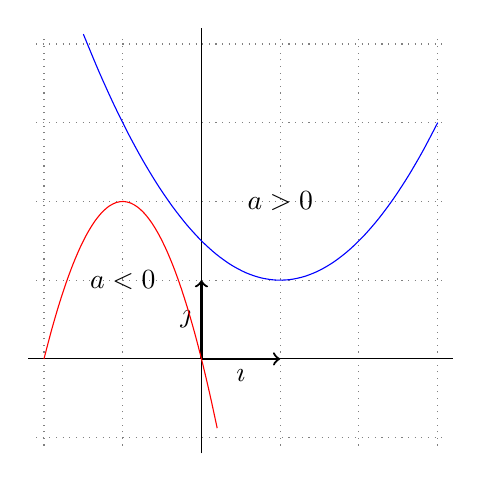
\begin{tikzpicture}
      \draw[dotted,color=gray] (-2.1,-1.1) grid (3.1,4.1);
      \draw[] (-2.2,0) -- (3.2,0);
      \draw[] (0,-1.2) -- (0,4.2);
      \draw[thick,->] (0,0) -- (1,0) node[midway,below]{$\vecteur\imath$};
      \draw[thick,->] (0,0) -- (0,1) node[midway,left]{$\vecteur\jmath$};
      \draw[domain=-1.5:3,smooth,blue] plot ({\x},{0.5*(\x+2)*(\x+2)-3*(\x+2)+5.5});
      \draw (-1,1) node{$a<0$};
      \draw[domain=-2:0.2,smooth,red] plot ({\x},{-2*\x*\x-4*\x});
      \draw (1,2) node{$a>0$};
    \end{tikzpicture}
  \end{center}
\end{propriete}

\begin{definition}
  On appelle \emph{sommet} le point qui correspond à l'extremum de la fonction. Il est situé sur l'axe de symétrie de la parabole, donc son abscisse est $-\frac{b}{2a}$.
\end{definition}

\subsection{Forme canonique}

\begin{propriete}
  Tout trinôme peut être mis sous la forme $f(x)=a(x-\beta)^2+\gamma$, où $\beta=-\frac{b}{2a}$. Cette forme s'appelle \emph{forme canonique}.
\end{propriete}
